
\begin{exercise}

% !TEX root = ../main.tex



[6 p. 92]  
\begin{minipage}[t]{.5\textwidth}
Een bal K gooi je vooruit en een bal L gooi je tegelijk naar beneden. Ze komen tegelijk aan in M. Met welke snelheid heb je bal L gegooid?
\end{minipage}
\hfill
\begin{minipage}[t]{.4\textwidth}
	\raisebox{1ex-\height}{%
		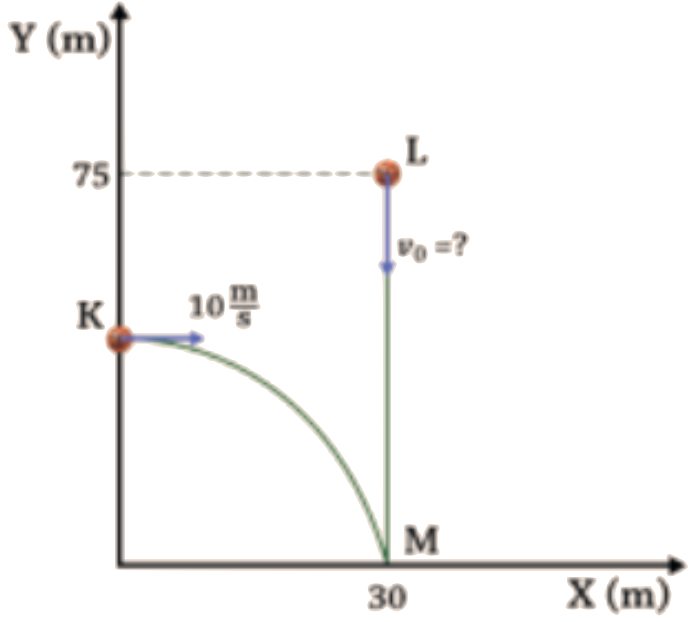
\includegraphics[width=\textwidth]{dyn/exercises/6p92}} 
\end{minipage}
\begin{oplossing}
% \newline
In horizontale zin voert bal K een ERB uit. Hij heeft dan ook 3 seconden nodig om M te bereiken. Die tijd is ook de valtijd voor L en kunnen we gebruiken om $v_0$ in verticale zin te bepalen. Uit $0=y_0+v_0t-\frac{1}{2}gt^2$ (de as staat omhoog gericht) vinden we 
\begin{eqnarray*}
v_0&=&\frac{\frac{1}{2}gt^2-y_0}{t}
\end{eqnarray*}
of $v_0=\SI{-10,29}{m/s}$. Merk op dat die beginsnelheid negatief is. De zin is tegengesteld aan de omhoog gerichte $y$-as.
\end{oplossing}

\end{exercise}
